
\subsection{Reveiwer Comments - \me{1}}

In this paper, the authors proposed a traffic aware resource allocation scheme for multi-cell MIMO-OFDM systems, where the precoders at all BSs are chosen to minimize the total user queue deviations. The problem is nonconvex and the authors proposed two centralized algorithms based on the successive approximation (SCA) technique to find a stationary point. Moreover, several distributed algorithms are also proposed using primal decomposition, alternating directions method of multipliers (ADMM), and decomposition via KKT conditions, respectively.

Most sections of this paper are well written. The results and algorithms also seem valid. However, the motivation of minimizing the total user queue deviations is not well justified. The convergence results of some algorithms are not clearly presented. The presentation of the distributed solutions needs significant improvement. Analysis and comparison of the signaling overhead and computational complexity between the centralized and distributed algorithms are also necessary to justify the advantages of distributed algorithms.

\resp We thank the reviewer for reading the paper and providing the comments. The response for the reviewer questions are made in line.

\subsection*{Detailed Comments}  
\cmnt{1} In Section II.B, please provides more justifications for the problem formulation in (6). For example, the Queue weighted sum rate maximization (Q-WSRM) is throughput optimal, i.e., if there exists a scheme which can make all queues stable, then the Q-WSRM can also do this. How about the proposed formulation in (6)? Is it also throughput optimal? 

\resp We fully agree with the reviewer comment. The Q-WSRM scheme is throughput optimal when the queues associated with the users are significantly large in comparison with the transmission rate (service rate). In order to restrict the over allocation of the available resources to a specific user beyond the total number of queued packets, we have included the additional rate constraint in the Q-WSRME algorithm. It would be ideal to compare with the Q-WSRME algorithm which performs similar to the Q-WSRM when the queued packets are large enough to be emptied by the current transmissions. Fig. \ref{fig-review} compares the centralized algorithms using average number of backlogged packets after \me{100} slots of transmission for different arrival rate. Note that the average arrival rate of all the users are same but the instantaneous arrivals are based on the Poisson distribution. It can be seen from Fig. \ref{fig-review} that the JSFRA scheme with \me{q=2} performs similar to the Q-WSRME scheme for higher arrival rates, which explains the dropping of the squared rate term in the Q-WSRM formulation. When the average arrival rate is smaller, the JSFRA scheme with \me{q=2} performs noticeably better than the Q-WSRME scheme as can be seen from the average number of backlogged packets. In all packet arrival scenarios, JSFRA scheme with \me{q=1} reduces the average number of backlogged packets over the given slots is lesser than the Q-WSRME scheme.
\begin{figure}
\centering
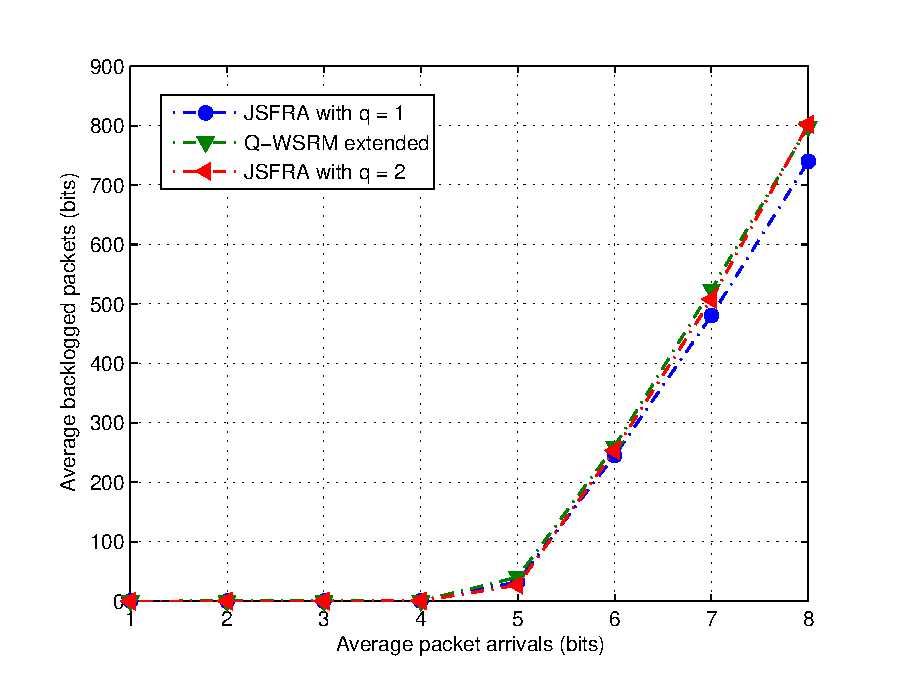
\includegraphics[width=\columnwidth]{Review/reviewer.eps}
\label{fig-review}
\caption{System \me{\lbrace N,N_B,K,N_R \rbrace = \lbrace 4,2,12,1 \rbrace}}
\end{figure}
The discussions are included in the Section \ref{time-correlated}.

\cmnt{2} Do the proposed solutions based on (6) achieve better average delay performance than the existing solutions? By the way, in the simulations, you should also add a figure comparing the average delay performance, instead of just comparing the performance metric defined by (6). This will better justify the advantage of the proposed solutions.

\resp We agree with the reviewer comment on the better average delay performance of Q-WSRM(E) approach over JSFRA scheme with \me{q=1} formulation. Note that the average delay can be reduced by including a convex minimum rate constraint in the JSFRA formulation to provide a guaranteed rate to all users or for certain users in the system. More over, the priority can also be incorporated easily in the formulation by the scaling factor \me{a_k} used in the formulation. As mentioned in Section \ref{sec-3.2}, the delay can also be addressed by using \me{q=2} or \me{q=\infty} norm objective in the JSFRA formulation.

\cmnt{3} In Section III.B, the convergence conditions under Algorithm 1 are not clear. First, you should be more specific about what is the SCA subproblem. Do you mean problem (19)? Second, does the uniqueness of the transmit and receive beamformers mean that the solution of the original problem in (16) is unique, or the solutions of the subproblems in (19) and (20) are unique, respectively?

\resp We understand the reviewer concerns. We have modified the convergence section to include additional information to provide more clarity. Appendix \ref{sec-3.5} discuss the convergence proof of the proposed algorithm in detail.

\cmnt{4} It is better to clearly summarize the convergence conditions and results (i.e., does it converge to a stationary point or the optimal solution) for all algorithms in a theorem/proposition.

\resp We agree with the reviewers view. We have updated the convergence proof to include the discussions on the stationary point and the optimal point.

\cmnt{5} At the end of Section III, you mentioned that the proposed reduced complexity resource allocation scheme is sensitive to the order in which the subchannels are selected for the optimization problem. Please provide a discussion how to choose this order.

\resp We thank the reviewer for the raising the concern on the selection order. We have elaborated the discussion on the sub-channel wise selection scheme in Section \ref{sec-3.4}. 

\cmnt{6} In the distributed algorithms, it is not clear what exact information is exchanged between the BSs or between the BSs and users. Moreover, the signaling overhead should be analyzed and compared with the centralized solution. The proposed distributed algorithms require exchanging over-the-air signaling or backhaul signaling for many times within each channel coherent time (e.g., from Fig. 2, the distributed algorithm requires 20-30 iterations to converge even when there are only 3 subchannels). I don’t think this is acceptable in practice. Is the signaling overhead of the distributed algorithm really smaller than the centralized algorithm which only requires exchange the CSI between the BSs for once within each channel coherent time?

\resp We thank the reviewer for the insightful comment on the practicality of the distributed algorithm. We fully agree with the reviewer comment on the information exchange between the BSs in the distributed approach. Please note that the proposed distributed algorithm based on the primal or dual decomposition is provided for the completeness purpose. Note that the distributed approach is performed for the convex subproblem, which leads to the same stationary point asymptotically as that of the centralized solution. In reality, we have to limit the number of iterations required for each distributed algorithm, thereby leading to a point which is not the stationary point when the algorithm is allowed to converge. In Section \ref{sec-4.3}, we have discussed a practical approach based on the KKT conditions, which attains a sub-optimal point with few number of iterations.

\cmnt{7} The convergence analysis of the distributed algorithms is not clear. For example, what is the exact condition to ensure the convergence of the distributed algorithms. Does the distributed algorithms also converge to a stationary point?

\resp We understand the reviewers concern. We have update the text on the convergence of the distributed algorithm (ADMM). Please not that the ADMM or the primal decomposition algorithm is used for the convex subproblem only. If the distributed algorithm is iterated until convergence, it is guaranteed to attain the same stationary point as that of the centralized algorithm \cite{boyd2011distributed}. We have included this discussion in Section \ref{sec-dist-conv}.

\cmnt{8} I’m totally confused with the ADMM approach in Section IV.A. Many notations, such as the local interference vector and consensus interference vector are used without formal definition. What is the difference between the local interference vector and consensus interference vector? What are their relationships with the actual interference vector. It seems that you are using the same notation for all of these interference vectors and I can’t tell when a notation refers to a local interference vector, a consensus interference vector, or the actual interference vector. These questions should be clarified and perhaps you should choose the notation system more carefully. For example, in (36), there are 3 similar notations and I don’t know which one is local interference vector and which one is the actual interference vector.

\resp We understand the concern of the reviewer. We have updated the distributed section to include all the details pointed by the reviewer.

\cmnt{9} In the distributed algorithms, it is not clear what information is available at each node. For example, what are your assumption on CSIT (CSI knowledge at each BS) and CSIR (CSI knowledge at each user)? How to 2 obtain the information used to perform the required calculation at each node (such as calculating the actual interference, MMSE receiver and the dual variables)?

\resp We understand the concern of the reviewer. We have updated the distributed section to include all the details pointed by the reviewer.

\cmnt{10} Do you have any convergence result for the proposed distributed solution based on the KKT conditions in Section IV.B? It seems that the iterative method to solve the KKT conditions is totally heuristic.

\resp We fully agree with the reviewer. It is a heuristic approach since we update the transmit precoder, receive beamformer and the dual variables all at each iteration. Please note that the proposed algorithm is of practical significance, since it has few number of iterations before the actual precoder design. It is surely not a stationary point of the original nonconvex problem but it is guaranteed to provide better performance in the sum rate compared to the distributed approaches presented in Section \ref{sec-4.1} and Section \ref{sec-4.2} for the same number of iteration. Note that, if the dual variables are allowed to iterate until convergence, the proposed KKT based scheme achieves the same stationary point for each fixed receive beamformer (similar to the distributed algorithms).

\cmnt{11} Since queue is a dynamic system evolving according to (3), it doesn’t make sense to compare the queue deviations at a given time. You should compare average queue deviations in the simulations. Moreover, you should also compare the average delay performance instead of just comparing the performance metric (queue deviations) defined in this paper. Using the queue deviations as the performance metric also needs more justification.

\resp We thank the reviewer for the insightful comment. We agree that the instantaneous deviation is not the right measure for the comparison. In the current work, we planned to discuss on the precoder design only and since the expectation is maximized by maximizing the function inside the expectation at each instant, we used the snapshot a given instant to compare different algorithms. Please note that Fig. \ref{fig-review} includes the comparison over \me{50} slot duration and plot compares the average number of backlogged packets. We thought of presenting the results with the time-correlated fading channel and the precoder design with fixed number of iterations in the future publication. If the reviewer still insist this figure needs to be included, we will include.

\cmnt{12} What is “SRA” in the simulation figures?

\resp We have updated the figure.

\cmnt{13} In the discussion for Fig. 1, you mentioned that JSFRA converge to the optimal point, and all algorithms are Pareto-optimal. Since the problem is non-convex, why these algorithm can find optimal solution or Paretooptimal point? 

\resp We thank the reviewer for the comment. We have updated the text to include pareto-suboptimal point.


\subsection*{Reveiewer comments - \me{2}}

\cmnt The logic from (6) to (16) is not clear. The only difference is the two newly introduced NON-CONVEX constraints (16b) and (16c), while the objective function (16a) and the constraint (16d) is the same as (6). The equivalence between (6) and (16) is not straightforward and it is confusing why the reformulation in (16) is beneficial.

\cmnt The authors use the successive convex approximation framework, but the approximate problem proposed by the authors is actually not convex. Inspecting (19), its objective function is the same as in (6), and the non-convexity of (6) comes exactly from the objective function, so (19) is not a convex problem. The same flaw is repeated several times in the approximate problems proposed by the authors.

\cmnt The authors proposed to use block coordinate descent method to solve (16). But as the authors have already pointed out, to apply block coordinate descent method, the constraint sets for different variables should be disjoint (uncoupled), which is however not the case in (16), because receive and transmit precoders (i.e w and m) are coupled in the constraints. It is confusing on its own why the authors made a statement that contradicts the proposed methodology, and the convergence followed is in question.

\cmnt Regarding the convergence of the SCA, the authors cited [27] for the convergence conditions, but the reference is wrong, because the conditions after the three bullets on page 6 are not mentioned in [27]. In case the authors disagree, please make the citation more specific, for example, specify the theorem/statement/proposition in [27] where those conditions are specified.

\cmnt The authors also cited [28] to establish the convergence of SCA. But the techniques of [27] and [28] are different, and the convergence conditions are different too. It is not clear why the authors need two set of convergence conditions for a single problem, and the resulting convergence analysis itself is not solid enough.

\cmnt Another comment on reference: to the reviewer's knowledge, the term SCA is never explicitly used in [2]. So please either correct the reference or be more specific (section, theorem, etc.).

\cmnt The authors propose primal decomposition method, ADMM approach to the non-convex problem (19), while their convergence analysis is based on literature that proved convergence for convex problems only, e.g., [13]. So the convergence analysis is not trustworthy.

\cmnt The length of the paper is too extensive. Some of the reformulations as mentioned in the previous comment can be skipped. Also, Section III.D. is not deeply explained and does not bring additional value to the paper. The implications of ordering the sub-channels for the iterative approach should be carefully studied and extensively explained in a different publication.

\cmnt Information regarding the value of q used to obtain the simulation results is missing (with exception of Fig. 3).

\cmnt In Fig. 1 and Fig. 2, the labels for the system model do not fit with the written description. Additionally, the reference scheme Q-WSRM is not optimal, since it over allocates resources if there are few queued packets. Therefore, it is not interesting for comparison purposes.

\cmnt Assuming that Fig. 2 and Fig. 3 where obtained based on the same simulation setup, i.e. user queues, number of transmit and receive antennas and number of base stations, it is not clear why results in Fig. 3 are worse than Fig. 2 when comparing JSFRA. Even more, since the number of sub-channels is larger in Fig. 3, the result seems contradictory.

\subsection*{Reveiewer comments - \me{3}}

\cmnt This manuscript focuses on the beamforming and scheduling optimization for IBC MIMO-OFDM system, including the centralized and decentralized optimization methods. This is an interesting and important topic.

\resp We thank the reviewer for reading the manuscript and providing valuable comments.

\cmnt 1. The number of transmitted packets \me{t_k}'s are optimization variables, which should be explicitly stated in the problem formulation of (6), (16), (19), (20) and (26) to avoid confusing.

\resp Please note that the objective function uses \me{v_k =  Q_k - t_k = Q_k - \sum_{n = 1}^N \sum_{l = 1}^{L} \log_2(1+\gamma_{l,k,n})} expression instead of including an additional constraint for the transmitted packets using the rate expression. It is necessary in case of the MSE formulation, where we have explicitly stated the optimization variable \me{t_k}. If the reviewer insist on replacing the rate expression using \me{t_k}, we can make those changes.

\cmnt 2. The manuscript states that the inequalities (16b) and (16c) achieve equality at optimality(line 23, page 5). This is not obvious. An easy case to check this statement is that assuming the system has two BS and each BS serves one user. When \me{Q_1=0} and 2nd BS has sufficiently large power, (16b) and (16c) do not hold equality. Rigorous proof is needed if authors stick to this statement.

\resp We thank the reviewer for the insightful comment. We modified the statement such that it is an under estimator for the actual SINR expression and will be tight when the system is limited by the transmit power.

\cmnt 3. The solution in (21) is obtianed for MMSE, i.e. for 2-norm(q=2). If \me{q=1} or \me{q=\infty}, it is actually an equivalent linear programming problem. Details for this solution should be provided.

\resp We thank the reviewer for the critical comment. We have update the manuscript to include the information about the receiver with other q values. Please note that the receive beamformer doesn't depend on the q value explicitly. It depends inherently through the transmit precoders.

\cmnt 4. The convergence proof need to be rigorous. The inequality of (23a) is opposite to the reference [28]. Also the statement on uniqueness of the transmit and the receive beamformers are not correct. Although we can choose one antenna to be real value, this does not mean the problem has unique solution!

\cmnt 5. (25) is generally wrong. (25) only holds when the MSE is minimized(by MMSE receiver) and the snr is the optimized(which is obtained by general eignvalue decompostion). This is clearly stated in the reference [5] and [6]. This can also be easily checked by comparing (25) and (2). Consequently the alternative formulation (26) based on this conclusion is questionable.

\resp We thank the reviewer for pointing out the information loss in the statement. We have provided more detail in the manuscript. The relation is valid if the receiver is based on the MMSE criterion. Note that, the receiver does not depend on the \me{q} value used in the objective. It depend only on the transmit precoders which in fact change based on the \me{q} value used in the objective function. 

\cmnt 6. For ADMM aproach, the determination of the value of \me{\rho} in equation (35a) should be discussed. 1. The numbers of transmitted packets for users  \me{t_k}'s are optimization variables. So they should be explicitly stated in the problem formulation (6), (16), (20) and (26) to avoid confusing.

\subsection*{Reveiewer comments - \me{4}}


\cmnt First, this reviewer is not convinced by the arguments for showing the convergence of the JSFRA method. "The SCA method" is often referred to, but never really defined or referenced. The three required conditions (as stated on p. 6, col. 1, rows 38-40) do not, as far as I can tell, appear in [27]. Indeed, [27] is concerned with optimization problems where the objective function is non-convex, but the constraint set is convex and separable over the blocks of variables. Perhaps you meant to cite [A], wherein non-convex constraints are handled in a similar way? Numerically, the algorithms do converge, and the argument put forward makes sense, but the treatment must be improved to be more rigorous.

\cmnt Second, the optimization problems formulated only depend on $Q_k$, the current levels of backlogged packets, and not on the arrival rates. This is due to how the conditional Lyapunov drift is minimized. This approach completely removes the queue dynamics from the optimization problem, essentially leading to greedy one-shot optimization in 7
every time instant. The framework would be more interesting if some sort of optimization (or tracking) is performed over several time instants, rather than the one-shot approach that is currently used for the JSFRA algorithms. Possibly, some expectation over the queues would be optimized then. Even if no analytical treatment of the tracking over several time-steps is added, I would at least highly recommend adding some simulation results where the proposed one-shot algorithms are performed sequentially over several time instants.

\cmnt Third, the distributed methods (at least the primal decomposition and ADMM) seem to be fairly straight-forward applications of existing results. This reviewer recommends spending more space on the convergence, than on the description of the distributed techniques. Still, it would be nice with a direct description of what local CSI is required, and how it is acquired, to perform the local computations for the primal decomposition and ADMM methods. For the description of the signaling of the CSI in Sec. IV-B, are you envisioning a TDD system?

\cmnt Finally, some readers might be confused by the "joint space-frequency" terminology, believing that the beamforming is performed over a joint space-frequency channel space, where the space-frequency channels are formed by block-diagonal matrices, each block belonging to one subcarrier. This could easily be clarified. 

\cmnt - p. 1, col. 1, row 42: "userss"

\resp Modified.

\cmnt - p. 1, col. 2, row 18: the precoders are used \_implicitly\_ as decision variables. This is the whole point, to avoid explicitly modeling the hard decisions in the optimization, and instead do soft decisions during the iterations, and then finally hard decisions after convergence.

\resp We thank the reviewer for the insightful comment on the proposed approach. We have modified the text accordingly.

\cmnt - p. 1, col. 2, row 33: Which chapter in [2] is referred to? With a quick look-through of the table of contents, I can't find and chapter or section treating the SCA method?

\resp We understand the reviewer's concern. We have provided the valid reference for the SCA scheme.

\cmnt - p. 2, col. 2, row 36: Write $\text{rank}(.)$ and $\min$ instead

\resp Changed.

\cmnt - p. 3, col. 1, row 26: It would be more clear to explicitly write out the dependence of $\mathbf{M}$ and $\mathbf{W}$ in $\tilde{v}$ here

\resp We thank the reviewer for the concern on the grouped variable. We have modified the expressions accordingly.

\cmnt - p. 3, col. 2, row 26: Which general MIMO-OFDM problem are you talking about here, and what is combinatorial about it? Is it the problem of selecting users to be served on orthogonal subcarriers? There is nothing inherently combinatorial over the problem in (6) as far as I can tell, as the beamformers are used as soft decision variables.

\resp We thank the reviewer for the comment. We have removed the word "combinatorial" from the text. 

\cmnt - p. 4, col. 2, row 40: "In fact, (5) provides similar expression of ..." This sentence is very hard to understand.

\resp It is restructured to include additional details.

\cmnt - (16d): suggest your write out the power constraints here, in order to be faster be able to interpret the optimization problem. There is hardly any spaced saved by referring back to (6b).

\resp Agreed.

\cmnt - p. 5, col. 1, rows 27-30: Here you might want to quickly mentioned how one could show the NP-hardness of (16).

\cmnt - p. 5, col. 1, row 50: "According to the SCA method...". I am not sure exactly how you define "\_the\_ SCA method"? Clarify or cite the definition.

\cmnt - p. 5, col. 2, row 31: Here is a case where it makes sense to reference earlier optimization constraints. However, are (19d) and (18) not the same??

\resp We thank the reviewer for pointing out the mistake. We have modified accordingly to the comment.

\cmnt - p. 5, col. 2, row 51: Slightly confusing with the notation between the iterates in (21b) and the MMSE filter in (22b).

\cmnt - p. 6, col. 1, row 9: You might want to add somewhere that (22b) can be used instead of the fixed-point of (21b), since the scaling of the receive filters do not matter in the SINRs. However, does it affect the convergence of the algorithm?

\cmnt - p. 6, col. 1, row 9: You might want to add somewhere that (22b) can be used instead of the fixed-point of (21b), since the scaling of the receive filters do not matter in the SINRs. However, does it affect the convergence of the algorithm?

\resp We thank the reviewer for the comment.

\cmnt - p. 6, col. 2, rows 8-10: I don't fully understand the reasoning on the relation between the constraint sets in the different iterations. Why is this the case?



\cmnt - p. 7, col. 1, row 35: Just because a problem is convex does not mean that it has a unique solution. (Although it seems to me that (26) should have a unique solution.) Is the problem in (26) strictly convex?

\resp We thank the reviewer for informing the important argument. The relaxed sub problem is strongly convex, due to the presence of norm function in the objective. Since the relaxation forced \me{q_{l,k,n} = 0}, the precoders are unique.

\cmnt - Table 1: "backpreassure"

\resp Changed in the revised manuscript

\cmnt - p. 11, col. 1, row 56: "performances". I'm not sure this is a countable noun.

\resp Changed in the revised manuscript

